
\documentclass[a4paper,12pt]{article}
\usepackage[a4paper, margin=2.4cm]{geometry}
\usepackage[utf8]{inputenc}
\usepackage{amsmath, amssymb} % Packages pour les maths
\usepackage[T1]{fontenc}
\usepackage{graphicx} 
\usepackage{caption}
\usepackage{setspace} % Espacement des lignes
\usepackage{tikz}





\begin{document}

\section{Modèle 1:}
\subsection{a. Bille remplie d'eau}

la terre perd de la température par rayonnement 

\[   P= \sigma T^4 
\]

\[    C \, \frac{dT}{dt} = - \sigma T^4 \, dt \times S
\]

\[\frac{dT}{dt} = - \frac{4 \pi R_T^2 \sigma T^4}{C}\]  

\textbf{Solution:} 
\[
T(t) = \left( \frac{C}{C/T_i^3 + 12\pi R^2 \sigma t} \right)^{1/3} 
= \frac{T_i}{\left(1 + 3k T_i^3 t \right)^{1/3}}
\]
avec \(k=\frac{4\pi R_T^2 \sigma}{C}\)
et \(C=c_{\text{m eau}}\times m=4,60 \cdot 10^{27} J\cdot K^{-1}\)

\bigskip

\textbf{hypothèse:} la Terre est assimilée à une boule d'eau de rayon \(R_{T}\) =Rayon de la Terre,  dans l'espace (le vide) sans atmosphère, sans soleil, avec une \(T_{\text{Terre}}\) une température de la Terre telle que  \(T_{\text{Terre}}\)> \(T_{\text{vide}}\), avec C=capacité massique de la Terre. 

\bigskip
\textbf{Modélisation:} 
    
    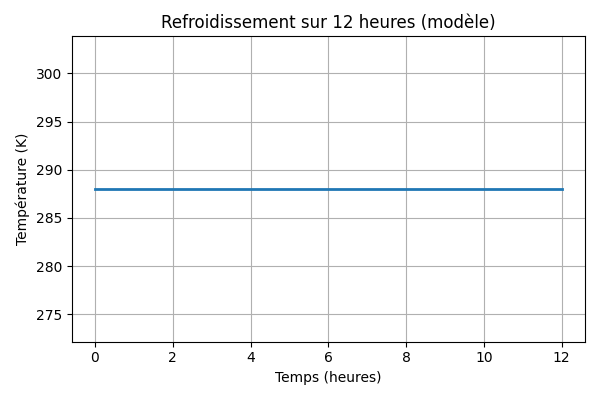
\includegraphics[width=0.8\linewidth]{../figures/modele1.png}
\\
\subsection{b. Coquille vide }
Puis on a améliorer le modèle en modélisant la Terre comme une coquille vide dont l'épaisseur est dr, ainsi on a recalculer la capacité thermique  \\

\begin{align*}
m &= \rho_{\text{eau}} \left( \frac{4}{3} \pi (R_T + dr)^3 - \frac{4}{3} \pi R_T^3 \right) \\
&\overset{DL}{\approx} \rho_{\text{eau}} \cdot 4\pi R_T^2 \cdot dr \\
\\
C &= c_{\text{eau}} \cdot \rho_{\text{eau}} \cdot 4\pi R_T^2 \cdot dr \\
&= 4{,}31 \cdot 10^{20} \ \text{J} \cdot \text{K}^{-1} \\
\\
k &= \frac{4\pi R}{c_{\text{eau}} \cdot \rho_{\text{eau}} \cdot 4\pi R^2 \cdot dr}
\end{align*}

    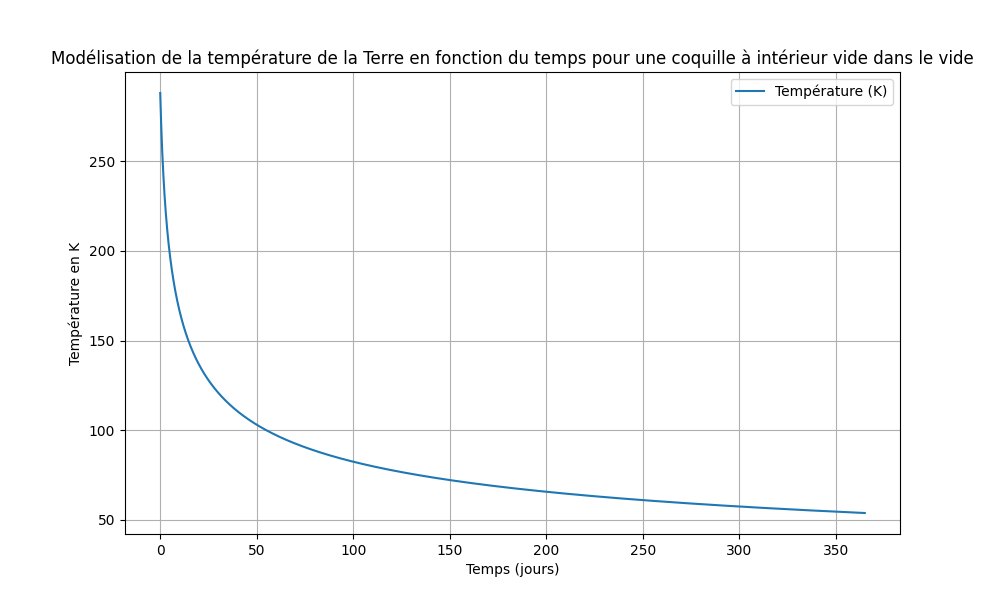
\includegraphics[width=0.8\linewidth]{../figures/modele1_coquille.png} 


\section{Modèle 2: Avec atmosphère}
\subsection{a. Boule d'eau avec atmosphère }
\section*{Équations de transfert thermique}

On introduira plus tard le \(P_{\text{th rayonnement}}\)

\begin{align*}
\delta Q &= c_{air}\, dT = -P_{\text{th,cond}} \cdot dt \\
\Rightarrow -\int \int \vec{j_{\text{th,cond}}}\, \vec{dS}\,dt = c_{air}\, dT \\
\Rightarrow -\int_{\theta=0}^\pi \int_{\phi=0}^{2\pi} h(T - T_0) \vec{e_{\text{r}}}\cdot r^2 \sin\theta\, d\theta\, d\varphi \vec{e_{\text{r}}}\, dt &=  c_{air}\, dT  \\
\Rightarrow -h(T - T_0) \cdot 4\pi\, dt &= c_{air}\, dT \\
\Rightarrow -T + T_0 = \frac{c}{h 4\pi} \frac{dT}{dt} \Rightarrow \frac{dT}{dt} &= -\frac{4\pi h}{c}(T - T_0)
\end{align*}

\vspace{0.5cm}
\textbf{hypothèse:}sysème de base l'astre entier assimiler à boule d'eau (résultat Elise)
coquille vide d'eau 
on assimile terre de température Tt avec eau, avec atmosphère avec température uniforme T  en ignorant la convection 
avec \(C_{\text{air}}\sim C_{\text{eau}}\)
avec  $T(t=0) = T_i$ 
$T(t \to +\infty) = T_0$  \ \ \ \
$T(t) = T_0 + (T_i - T_0)e^{-kt}$ \quad avec $k = \frac{4\pi h}{c}$
modèle sans coquille 
modèle coquille (figure gitub)

modèle 3 : modèle 1 + modèle 2 avec intérieur non vide 

 
\vspace{1cm}


\end{document}
